\newpage
\section{FFT of FID}

\lstinputlisting[style=Matlab-editor, basicstyle=\small, caption={Slide 17.}, label={lst: exp_lorentz}, firstline=2]{./codigo/fft_fid1.m}

\begin{figure}[!ht]
    \centering
    \begin{minipage}[b]{0.49\textwidth}
        \centering
        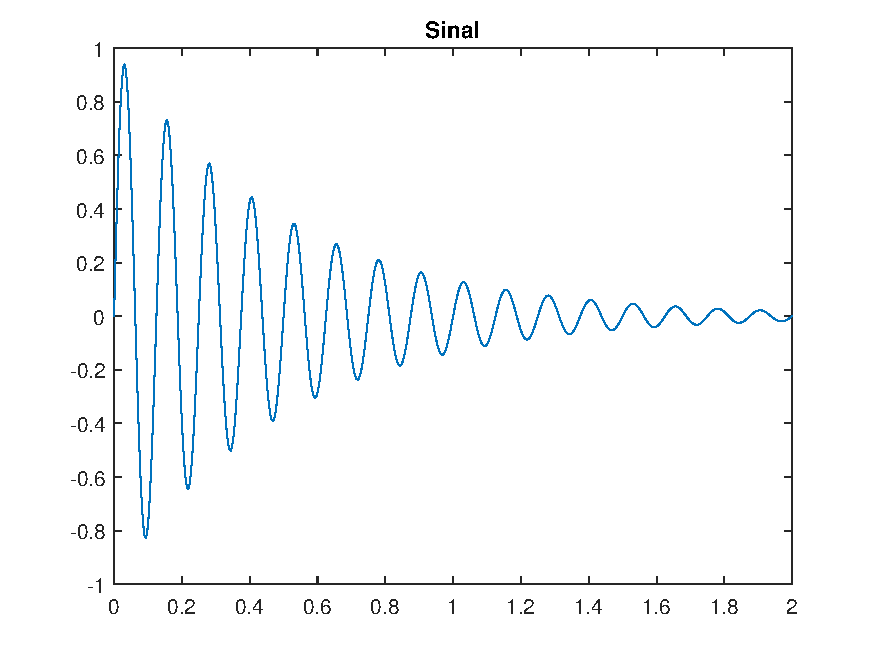
\includegraphics[width=\textwidth]{fft_fid1.1.pdf}
    \end{minipage}
    \hfill
    \begin{minipage}[b]{0.49\textwidth}
        \centering
        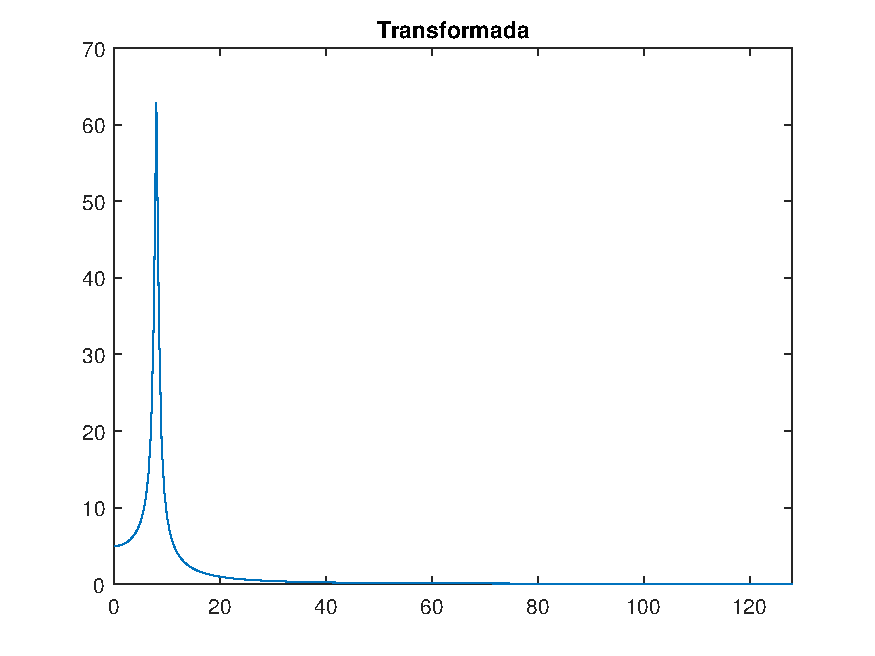
\includegraphics[width=\textwidth]{fft_fid1.2.pdf}
    \end{minipage}
    \caption{FFT of FID 1.}
\end{figure}

\newpage

\lstinputlisting[style=Matlab-editor, basicstyle=\small, caption={Slide 18.}, label={lst: exp_lorentz}, firstline=2]{./codigo/fft_fid2.m}

\begin{figure}[!ht]
    \centering
    \begin{minipage}[b]{0.49\textwidth}
        \centering
        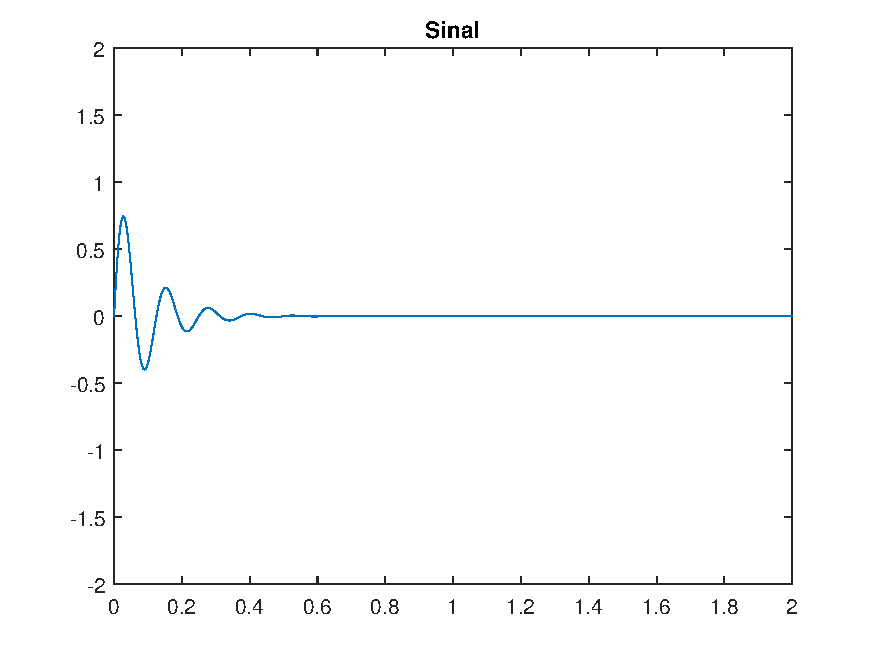
\includegraphics[width=\textwidth]{fft_fid2.1.pdf}
    \end{minipage}
    \hfill
    \begin{minipage}[b]{0.49\textwidth}
        \centering
        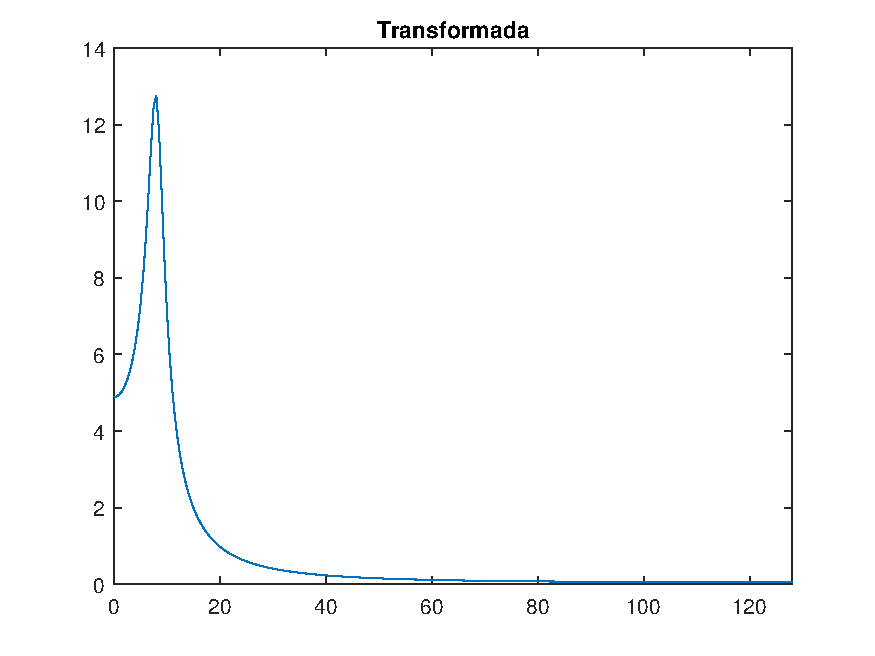
\includegraphics[width=\textwidth]{fft_fid2.2.pdf}
    \end{minipage}
    \caption{FFT of FID 2.}
\end{figure}

\newpage

\lstinputlisting[style=Matlab-editor, basicstyle=\small, caption={Slide 19.}, label={lst: exp_lorentz}, firstline=2]{./codigo/fft_fid3.m}

\begin{figure}[!ht]
    \centering
    \begin{minipage}[b]{0.49\textwidth}
        \centering
        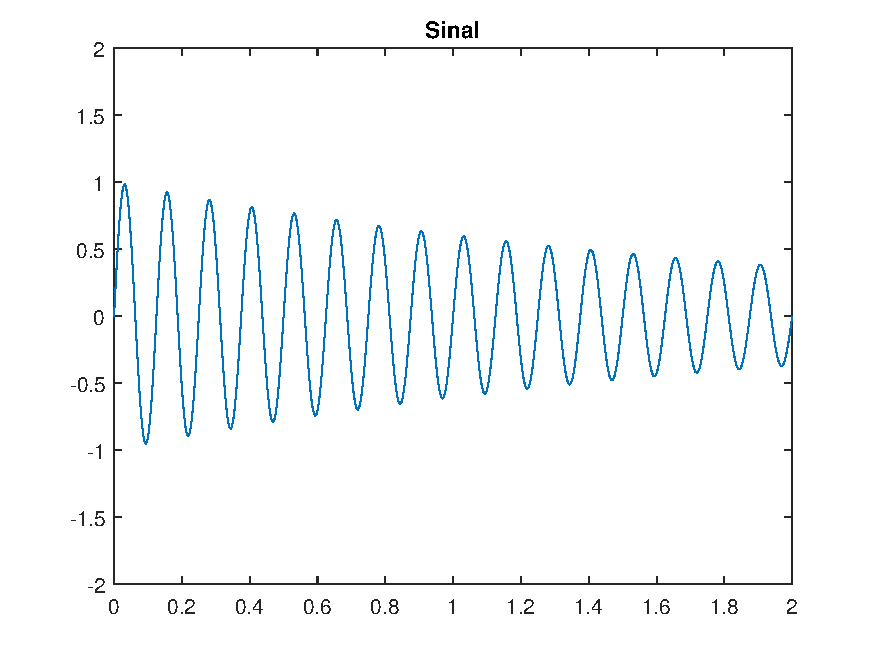
\includegraphics[width=\textwidth]{fft_fid3.1.pdf}
    \end{minipage}
    \hfill
    \begin{minipage}[b]{0.49\textwidth}
        \centering
        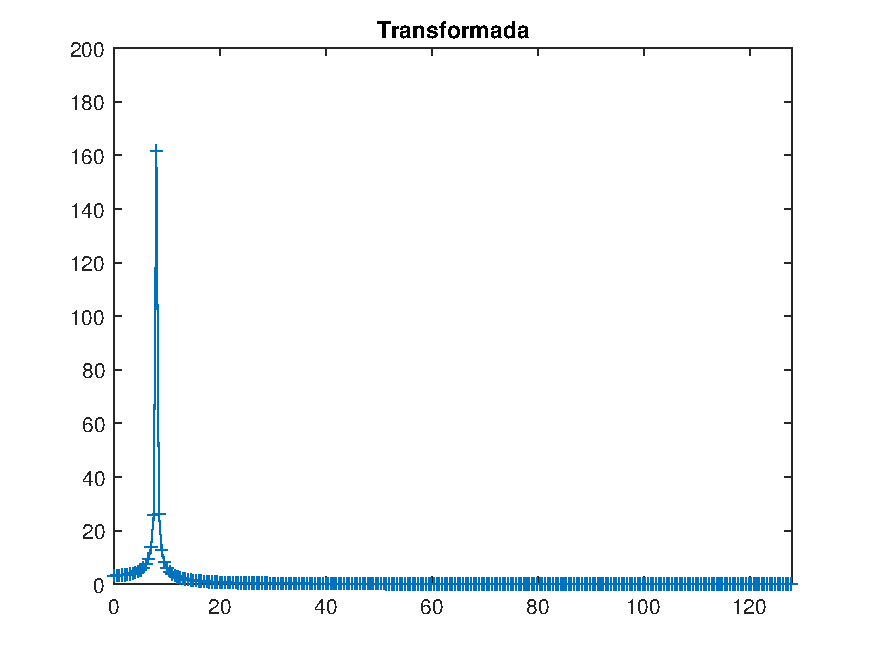
\includegraphics[width=\textwidth]{fft_fid3.2.pdf}
    \end{minipage}
    \caption{FFT of FID 3.}
\end{figure}

\newpage

\section{Efeito de mudar a taxa de amostragem}

\lstinputlisting[style=Matlab-editor, basicstyle=\small, caption={Slide 21.}, label={lst: exp_lorentz}, firstline=2]{./codigo/fft_fid4.m}

\begin{figure}[!ht]
    \centering
    \begin{minipage}[b]{0.49\textwidth}
        \centering
        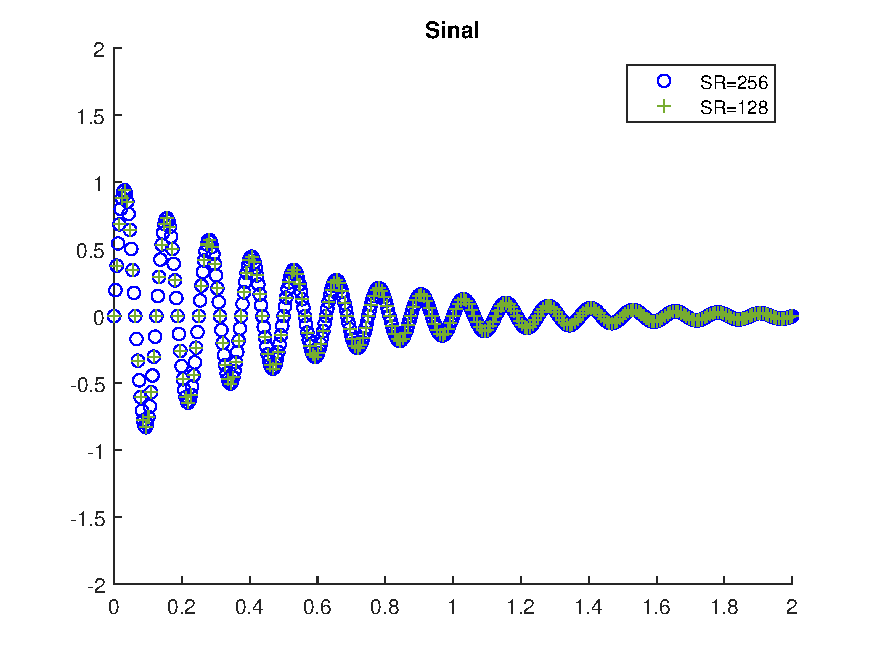
\includegraphics[width=\textwidth]{fft_fid4.1.pdf}
    \end{minipage}
    \hfill
    \begin{minipage}[b]{0.49\textwidth}
        \centering
        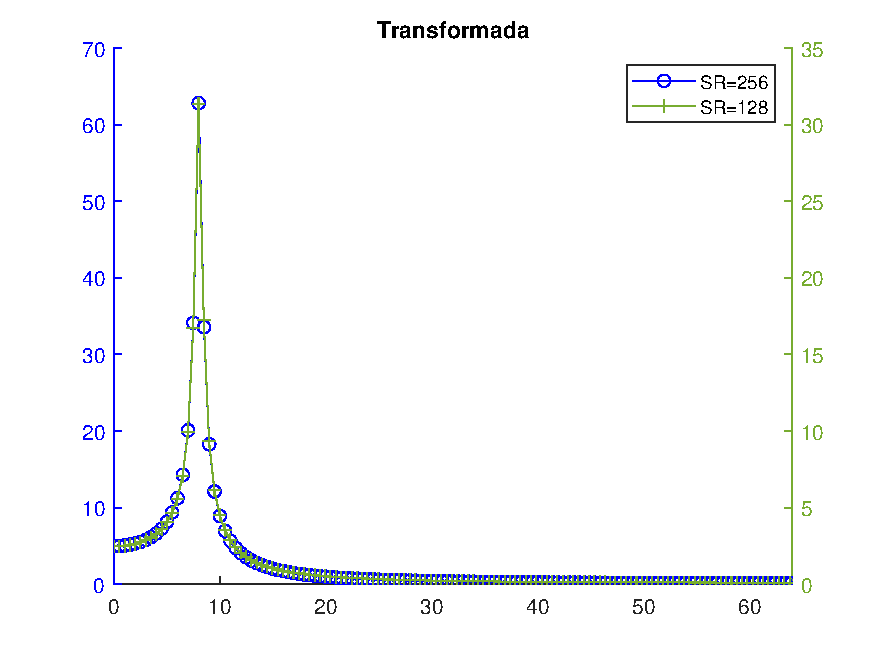
\includegraphics[width=\textwidth]{fft_fid4.2.pdf}
    \end{minipage}
    \caption{Diferentes sampling rates.}
\end{figure}

\section{Efeito de mudar a duração de amostragem}

\lstinputlisting[style=Matlab-editor, basicstyle=\small, caption={Slide 24.}, label={lst: exp_lorentz}, firstline=2]{./codigo/fft_fid5.m}

\begin{figure}[!ht]
    \centering
    \begin{minipage}[b]{0.48\textwidth}
        \centering
        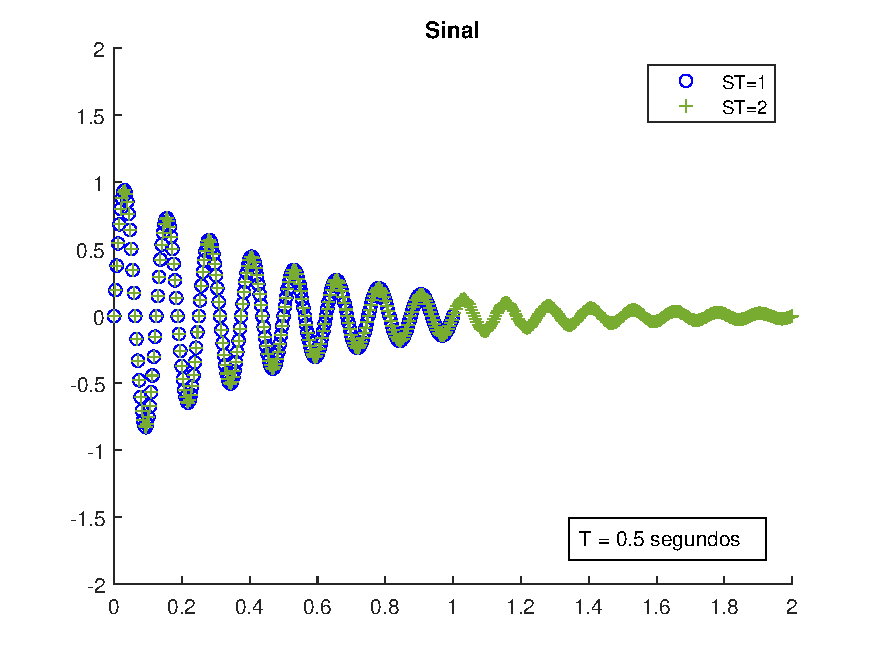
\includegraphics[width=\textwidth]{fft_fid5.1.pdf}
    \end{minipage}
    \hfill
    \begin{minipage}[b]{0.48\textwidth}
        \centering
        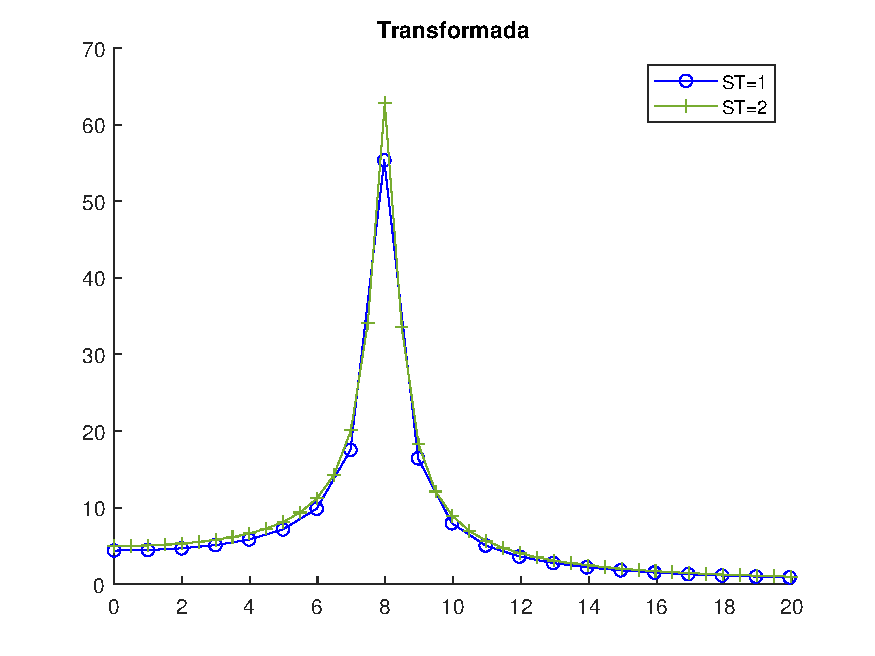
\includegraphics[width=\textwidth]{fft_fid5.2.pdf}
    \end{minipage}
    \caption{Duração de amostragem, T = 0.5 segundos.}
\end{figure}

\begin{figure}[!ht]
    \centering
    \begin{minipage}[b]{0.48\textwidth}
        \centering
        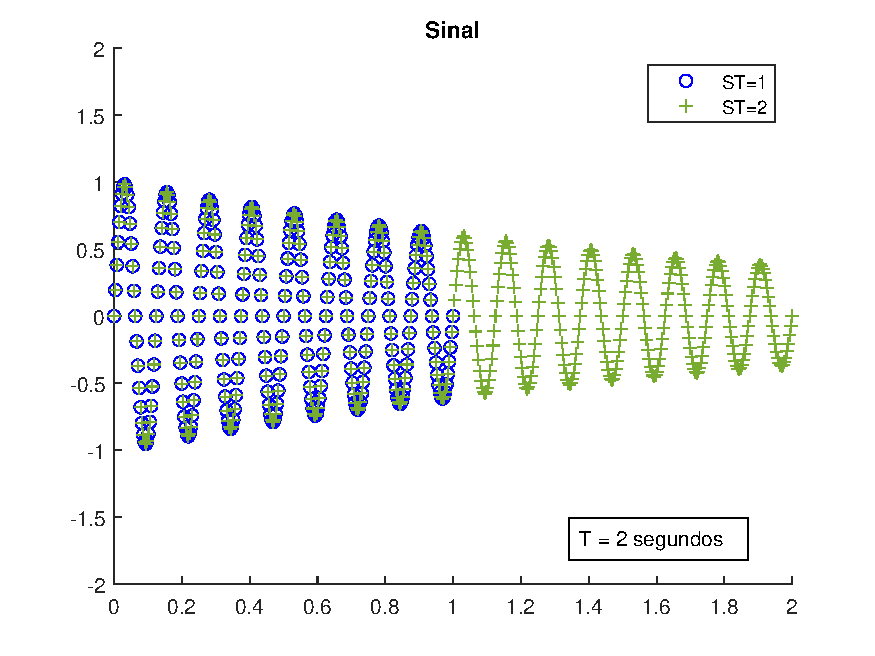
\includegraphics[width=\textwidth]{fft_fid6.1.pdf}
    \end{minipage}
    \hfill
    \begin{minipage}[b]{0.48\textwidth}
        \centering
        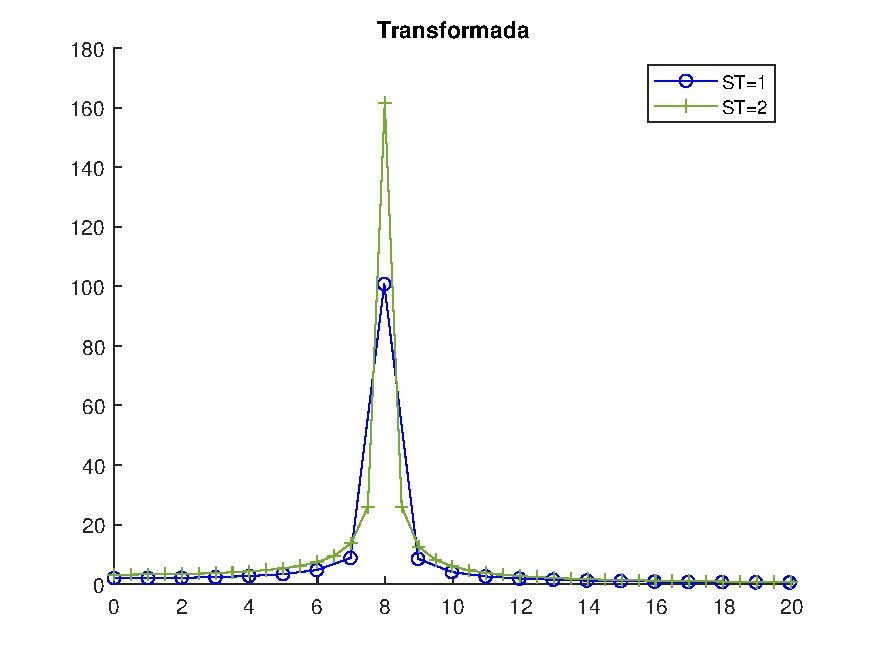
\includegraphics[width=\textwidth]{fft_fid6.2.pdf}
    \end{minipage}
    \caption{Duração de amostragem, T = 2 segundos.}
\end{figure}

\begin{figure}[!ht]
    \centering
    \begin{minipage}[b]{0.48\textwidth}
        \centering
        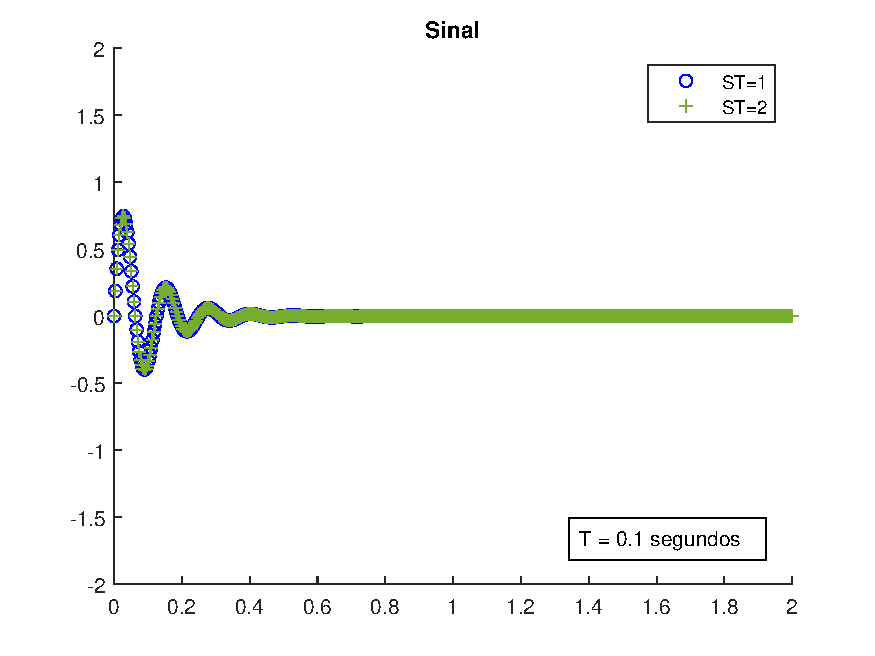
\includegraphics[width=\textwidth]{fft_fid7.1.pdf}
    \end{minipage}
    \hfill
    \begin{minipage}[b]{0.48\textwidth}
        \centering
        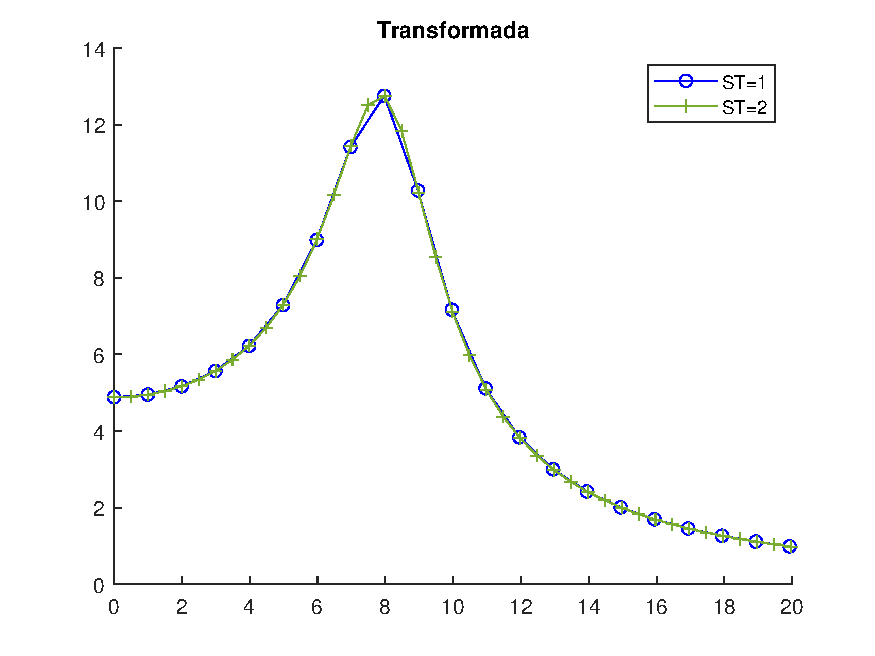
\includegraphics[width=\textwidth]{fft_fid7.2.pdf}
    \end{minipage}
    \caption{Duração de amostragem, T = 0.1 segundos.}
\end{figure}

\newpage

\section{Múltiplas frequências}

\lstinputlisting[style=Matlab-editor, basicstyle=\small, caption={Slide 28.}, label={lst: exp_lorentz}, firstline=2]{./codigo/multiplefreq.m}

\begin{figure}[!ht]
\centering
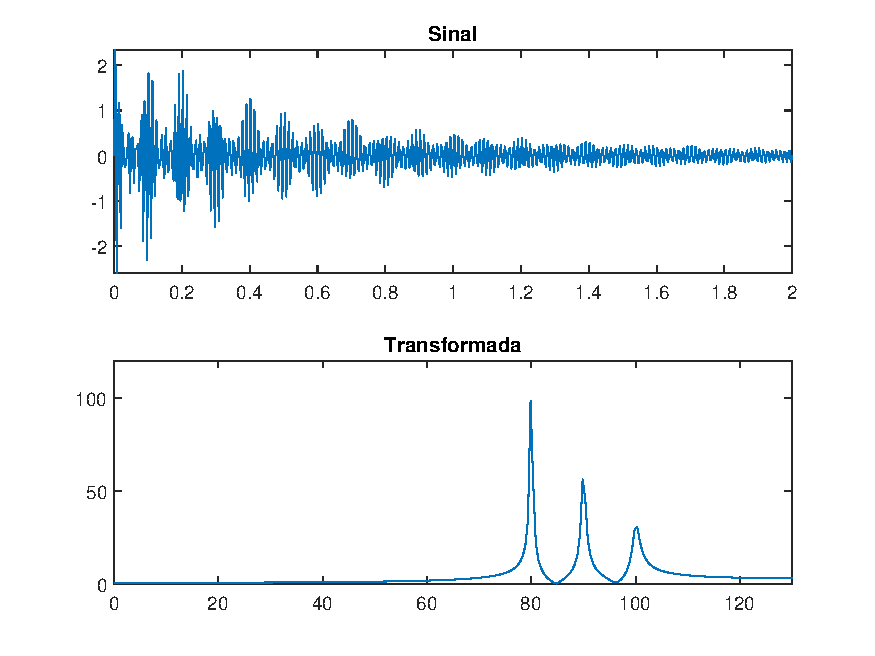
\includegraphics[width=0.75\textwidth]{multiplefreq1.pdf}
\caption{Múltiplas frequências (1).}
\end{figure}

% \begin{figure}[!ht]
%     \centering
%     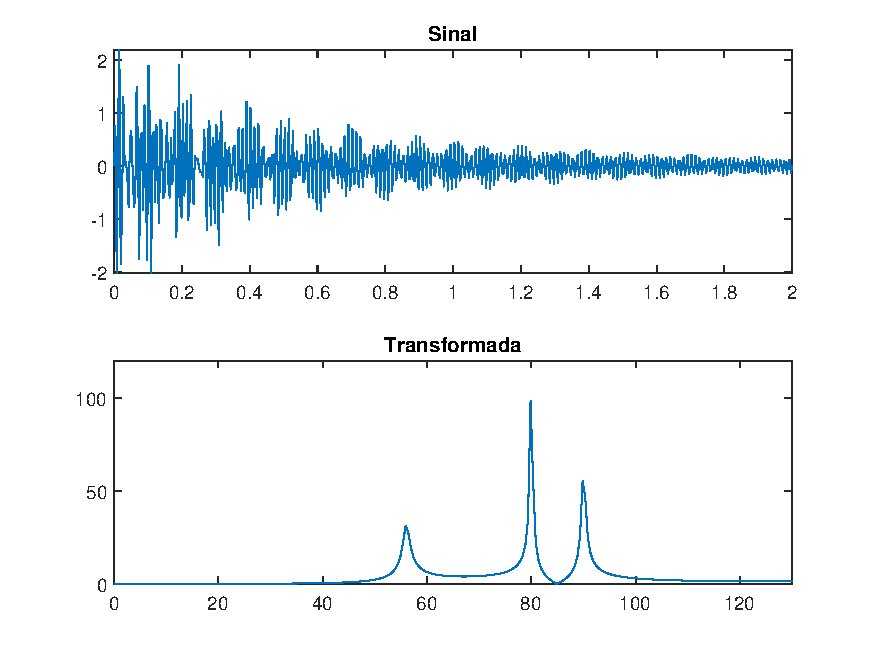
\includegraphics[width=0.75\textwidth]{multiplefreq2.pdf}
%     \caption{Múltiplas frequências (2).}
% \end{figure}